\begin{solution}
The maximum amount of rainfall is 120 millimeters.\\[0.2cm]

One scenario for 120 millimeters of rainfall is that 10 millimeters fall in each of the following intervals (numbers are in minutes):

[0,10], [60,70], [70,80], [130,140], [140,150], [200,210], [210,220], [270,280], [280,290], [340,350], [350,360], [410,420]

The following figure shows the time intervals for the first 6 rainfall intervals and the corresponding basins. The rest of the intervals (from minute 210 onwards) and the basins are placed similarly. Each 10-millimeter rainfall is shown by a blue square. The intervals of the 6 basins are also shown at the bottom of the diagram. As you can see, exactly 10 millimeters of rain falls in each basin.

\begin{center}
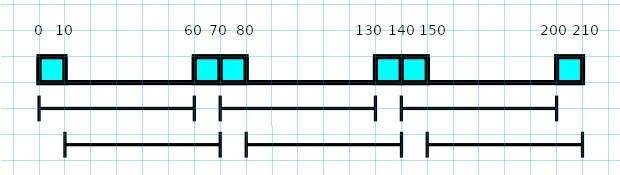
\includegraphics[width=10cm]{79/figs/79_0.jpg}
\end{center}

In the following, we show that the total amount of rain is bounded by 120 millimeters.

\begin{lemma}\label{lm:1}
In a one-hour interval, at most 20 millimeters of rain can fall.
\end{lemma}
\begin{proof}
Suppose for the sake of contradiction that more than 20 millimeters of rain falls in a one-hour interval. Consider a moment in time when slightly more than 10 millimeters of rain has fallen but there is still more than 10 millimeters of rain remaining until the end of the interval. The basin that is outside at this moment must either include all the rainfall from this moment until the end of the interval or all the rainfall from the beginning of the interval to this moment, both of which are more than 10 millimeters, which contradicts the problem conditions. Therefore, the initial assumption is false, and there is no one-hour interval in which more than 20 millimeters of rain falls.
\end{proof}

Also note that at each moment in time there should be a basin collecting rain, thus there is a basin that collects the rain in the first hour and there is a basin that collects rain in the last hour. Thus, in each of the first and last hours, at most 10 millimeters of rain has fallen. This in addition to Lemmas proves that the total rainfall is at most $2\cdot10+5\cdot20=120$ millimeters.
\end{solution}
